\documentclass[conference]{IEEEtran}

\usepackage{amsmath}
\usepackage{algorithm}
\usepackage{algpseudocode}
\usepackage{graphicx}
\usepackage{tipa}
\usepackage{flushend}

\makeatletter
\def\BState{\State\hskip-\ALG@thistlm}
\makeatother

\newcommand{\argmax}{\arg\!\max}

% correct bad hyphenation here
\hyphenation{op-tical net-works semi-conduc-tor}

\begin{document}

\title{Analyzing and Classifying Indonesian Spontaneous and Dictated Speech}

\author {
    \IEEEauthorblockN {
        Cil Hardianto Satriawan\IEEEauthorrefmark{1},
        Dessi Puji Lestari\IEEEauthorrefmark{2}
    }
    \IEEEauthorblockA {
        School of Electrical Engineering and Informatics\\
        Bandung Institute of Technology\\
        Bandung, Indonesia 40132\\
        \IEEEauthorrefmark{1}23515053@std.stei.itb.ac.id,
        \IEEEauthorrefmark{2}dessipuji@stei.itb.ac.id
    }
}

\maketitle

\begin{abstract}
The accurate recognition of spontaneous speech is crucial in achieving practical speech recognition.
Statistical-based recognition models typically employ a large amount of read or dictated speech for training, which often yields poor spontaneous recognition performance.
Many approaches have been forwarded to improve performance, including model adaptation and model switching.
In an effort to improve Indonesian language spontaneous recognition performance, we attempt to pinpoint the acoustic differences between spontaneous and dictated Indonesian speech.
At the phoneme level, we find that there are differences in the distribution and pronunciation of several key phonemes associated with filled pauses.
Across speakers, there is a consistent reduction in segment duration and segment energy, with a less marked spectral reduction.
Using these differences as a starting point, we train a number of classifiers that can accurately identify spontaneous and read Indonenesian utterances at F1 scores consistently above 90\%.
We show that classification is achievable by considering segment features and feature differences between consecutive segments, or "delta" and "delta-delta segments".
\end{abstract}

\begin{IEEEkeywords}
Speech recognition, spontaneous speech, Indonesian language
\end{IEEEkeywords}

\IEEEpeerreviewmaketitle

\section{Introduction}
The accurate recognition of spontaneous speech is one of the large ongoing challenges towards achieving practical speech recognition, with many systems still performing poorly.
This is seemingly in contrast to the recognition performance achievable on most state-of-the-art statistical-based systems on dictated speech tasks and limited domain spoken interactions \cite{furui2}.

This poor performance may be attributed in part to the fact that a large proportion of the data used to train models is derived from dictated instead of spontaneous speech.
Recording and labelling large amounts of new spontaneous speech is a difficult and costly process, whereas existing Indonesian language resources are scarce or non-existant \cite{hoesen}.
In addition, although spontaneous recognition is an important component of practical speech recognition, research has only relatively recently shifted in this direction.

Spontaneous and dictated speech also differ in various ways.
It has been proposed that spontaneous speech is less ordered both linguistically and acoustically \cite{furui2}, and differs spectraclly from dictated speech \cite{nakamura}.
Spontaneous speech contains filled pauses, repairs, hesitations, repetitions, and disfluencies, which are largely absent in dictated speech.
The exact differences vary by language, with some languages exhibiting a strong tonal difference between spontaneous and dictated speech \cite{dellwo}.

A number of methods have been developed to improve spontaneous speech recognition performance.
In the model adaptation approach, a large amount of dictation data is adapted to a small amount of spontaneous data while training the acoustic model, using a method such as Maximum A Priori (MAP) adaptation.
In the second approach, acoustic and language models for spontaneous and dictated speech are trained separately, with a method to switch or weigh models on the fly.
Model switching relies on a reliable way to differentiate between spontaneous and dictated speech that is independent of the specific acoustic models.

In either case, it is instructive to understand how acoustic differences between spontaneous and dictated speech manifest and how to describe them.
With a better understanding of these differences we can train better specialized models for spontaneous or mixed speech, for example utilizing the model switching approach.
The goal is to achieve a reasonably performant "front-end" classifier that can pass data to a number of back-end models specialized for the task at hand.

In the following section we describe the relevant literature and the speech corpus used for analysis.
We then discuss at length the various phoneme-level differences between spontaneous and read speech in the Indonesian language.
Finally we attempt to engineer segment-level acoustic features and utilize the feature set to classify segmented utterances.

\section{Related Works}

In classifying spontaneous speech, a number of approaches may be taken.
Many studies have focused on linguistic features such as grammar, word choice, hesitations, speech rate, pause types, pause structures, intonation, and articulation \cite{barik}\cite{blaauw}\cite{umeda}.
While such features are able to describe the semantic and syntactic characteristics of spontaneous speech, they are limited by the difficulty of labeling the training data.
Acoustic characteristics of spontaneous speech, on other hand, are easier to extract, but more difficult to use for classification purposes \cite{nakamura}.
Furui has shown that there is a substantial difference in the spectral properties of vowels between read and spontaneous speech \cite{furui1}.
By taking the differences between phoneme vectors of varying styles and their respective centers/averages, the spectral reduction of various phonemes between various speaking styles can be meaningfully distinguished.
A very promising new approach is in extracting the GMM supervectors between multiple utterances \cite{asami}, though this is limited by the latency of the classification results.

The exact definition of what constitutes "spontaneous" speech may often make or break a particular method.
For spontaneous speech that is different from read speech only in terms of preparedness of speech, but controlling for factors such as intonation, pitch, and speaking rate, it is very difficult even for humans to distinguish between the two \cite{laan}.
An oft-proposed approach to characterizing spontaneous speech is the use of prosodic features that describe the intonation and rhythm of speech \cite{silverman}.
An indirect approach, through the attempt to classify multiple classes, may shed more light into the issues involved \cite{liu}.

Specifically with regards to Indonesian, recent advances have been made in building large scale systems \cite{lestari}\cite{sakti}.
However problems still persist with regards to spontaneous speech.
Hoesen et al., building on previous Indonesian language model adaptation work\cite{lestari2}, have developed a reasonably performant Indonesian language speech recognition system, capable of achieving upwards of 80\% accuracy for dictated speech but only around 65\% for spontaneous speech, even with model adaptation.
Methods using general machine learning algorithms have been proposed for handling filled pauses in Indonesian \cite{sani}.

Detecting spontaneous and read utterances based on unlabelled segments relies on achieving reliable speech segmentation.
Many methods have been described in the literature to achieve this, building on the standard Hidden Markov Model (HMM) approach or using newer unsupervised approaches \cite{scharenborg}.
For this work, the Kaldi speech toolkit \cite{povey} is used primarily for speech segment extraction and obtaining the per frame MFCC features of recordings.

\section{Speech Corpus}

The Perisalah Corpus is a collection of spontaneous and read speech recorded for the development of the Perisalah Speech Recognition System in collaboration with PT. Inti, an Indonesian public telecommunications company.
The corpus samples a variety of different age groups and local dialects.
The meeting transcription system is being deployed at various government institutions at the national and regional levels.
The read/dictation part of the corpus was build to be lexically balanced with respect to written Indonesian.

\subsection{Corpus Overview}

After cleaning, the corpus consists of 297 native Indonesian speakers, with on average 275 dictated and 61 spontaneous utterances per speaker, totalling 81240 dictated and 18210 spontaneous utterances, respectively.
On average, dictated utterances are 6.54 seconds long and spontaneous utterances 8.33 seconds long for a total of 147.6 and 42.1 hours of dictated and spontaneous speech, respectively.

Demographically, speakers were taken from both genders roughly equally, with 143 male speakers and 154 female speakers.
Fig. \ref{demographics1} shows the distribution of genders across dialects, the sampled dialects being Javanese (J), Sundanese (S), Minanga (M), Batak (T), Betawi/Melayu (A), Balinese (B), Sulawesi (W), and Maluku/Papua (P).
Roughly 57\% of Indonesians live on Java, where the Javanese, Sundanese, and Betawi/Melayu dialects originate.
Two age groups were defined; ages 40 years and under, and ages above 40 years, with 243 and 53 speakers, respectively.

\begin{figure}[!htb]
\centering
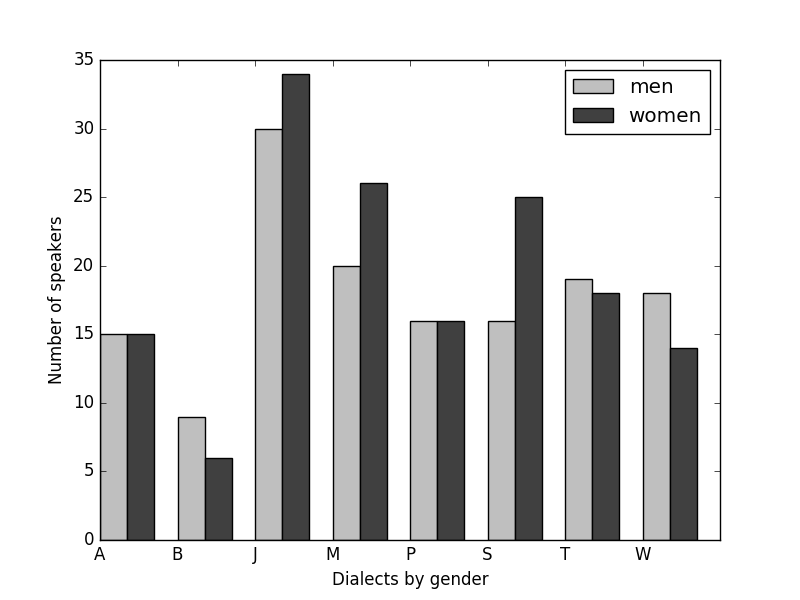
\includegraphics[width=3.3in]{demograph}
\caption{Number of members of each gender for each dialect}
\label{demographics1}
\end{figure}

Utterances for prepared texts were taken from newspaper articles and magazines, and hence derived from real-world examples, albeit written ones.
A total of ten different sets were compiled, labelled from 'A' to 'J'.
Speakers were recorded in a single session, with read speech recorded first and spontaneous speech afterwards.
For spontaneous speech, speakers were asked to choose an arbitrary topic in which they were comfortable with and thus asked to speak at length about it.

Fluency of speech varies greatly within the corpus, with some participants experiencing difficulties reading fluently, while others were highly uncomfortable when told to improvise a topic.
Utterances for spontaneous speech were segmented by hand; that is, the start and end of sentences is dependent on the studio operator's comprehension of the speech, although supervision was provided.
Hence, using the duration of utterances as a metric should be done with caution.

\subsection{Acoustic feature extraction}

Speech audio data is represented as audio samples taken at a particular rate.
A constant number of possibly overlapping audio samples are processed in a frame to obtain low level spectral, cepstral, and energy features.
A segment, comprised of a varying number of such frames, represents a single phoneme.
For the purposes of our acoustic analysis, linguistic units other than the phoneme are ignored and we instead consider utterances as sequences of segments.
In addition to frame and segment-level acoustic information a number of high level features are obtained at the utterance and speaker levels, namely the specific speaker of an utterance, their gender, dialect, and age.

Segments are force aligned on a prebuilt HMM trained using the Kaldi toolkit.
The segment duration, location and phone are obtained for each utterance in the corpus.
171 phones are defined in the corpus, which includes voiced and spoken phones, fillers, silence, and other non-speech phones.
The 64 most common phones calculated by frequency of appearance in the corpus are displayed in Table \ref{phones}.
These phones account for 98.15\% of the segment occurences in the corpus.
Spoken phones are further separated as belonging to the beginning, inside, or end of a word, indicated by a 'B', 'I', and 'E' suffix, resepectively.
The '@' symbol represents the phonetic '\textipa{@}'.

\begin{table}[!htb]
\renewcommand{\arraystretch}{1.3}
\caption{Common phones}
\label{phones}
\centering
\begin{tabular}{|c|c|c|c|c|c|c|c|}
    \hline
    @\_B & @\_E & @\_I & a\_B & a\_E & a\_I & b\_B & b\_I\\
    \hline
    c\_B & c\_I & d\_B & d\_I & e\_B & e\_I & f\_B & f\_I\\
    \hline
    g\_B & g\_I & h\_B & h\_E & h\_I & i\_B & i\_E & i\_I\\
    \hline
    j\_B & j\_I & k\_B & k\_E & k\_I & l\_B & l\_E & l\_I\\
    \hline
    m\_B & m\_E & m\_I & n\_B & n\_E & n\_I & ng\_E & ng\_I\\
    \hline
    ny\_I & o\_B & o\_E & o\_I & p\_B & p\_E & p\_I & r\_B\\
    \hline
    r\_E & r\_I & s\_B & s\_E & s\_I & sil & t\_B & t\_E\\
    \hline
    t\_I & u\_B & u\_E & u\_I & w\_B & w\_I & y\_B & y\_I\\
    \hline
\end{tabular}
\end{table}

For each frame, the formants and MFCCs are extracted.
The first four formants of each frame are calculated by solving its Linear Predictive Coefficients (LPC) an alignment subroutine.
The first 13 MFCCs are obtained during the pretraining of the segmentation HMM through the Kaldi toolkit, using the training defaults including Cepstral Mean Subtraction (CMS).
The delta and delta-delta features were calculated manually during frame alignment.
Apart from averaged frames, features at the segment level include segmental duration and location, and segment label in terms of phoneme.
The complete list of features is shown in Table \ref{features}.

\begin{table}[!htb]
\renewcommand{\arraystretch}{1.3}
\caption{Acoustic features}
\label{features}
\centering
\begin{tabular}{|l|r|r|r|r|r|}
    \multicolumn{1}{c}{} \textbf{Segment-level features}\\
    \hline
    Cepstral (36) & MFCC 12 + $\Delta$12 + $\Delta\Delta$12\\
    \hline
    Log energy (3) & MFCC 1 + 1$\Delta$ + 1$\Delta\Delta$\\
    \hline
    Temporal (2) & Duration 1 + Position 1\\
    \hline
    Spectral (4) & Formants 4 F0 - F4\\
    \hline
    \multicolumn{1}{c}{} \textbf{Utterance-level features}\\
    \hline
    Utterance ID (1) & Utterance number\\
    \hline
    Label (1) & Spontaneous or dictated\\
    & 'Z' for spontaneous or\\
    & one of 'A' - 'J' for dictated\\
    \hline
    \multicolumn{1}{c}{} \textbf{Speaker-level features}\\
    \hline
    Speaker ID (1) & Speaker number\\
    \hline
    Gender (1) & Female or male\\
    \hline
    Dialect (1) & Jawa (J), Sunda (S)\\
    & Minang (M), Batak (T)\\
    & Betawi/Melayu (A)\\
    & Bali (B), Sulawesi (W)\\
    & or Maluku/Papua (P)\\
    \hline
    Age group (1) & Young (M) or old (L)\\
    \hline
\end{tabular}
\end{table}

\subsection{Phone analysis}

The analysis of data that follows is primarily exploratory, focusing on phone-level differences and with the secondary goal of obtaining feature configurations that maximizes the distance between spontaneous and dictated speech.
In this section the data is unnormalized unless where stated to allow for easier interpretation.

A high level view of the data is obtained by first grouping phones into spontaneous and dictated classes and subsequently averaging the segment features in both groups over all utterances and speakers.
This view is filtered such that only phones of frequencies above 0.001\% in both dictated and spontaneous scenarios are processed further; for a typical speaker, this amounts to six spontaneous occurences of that phone in total.
From this view, differences in phone frequency and average duration per phone between spontaneous and dictated speech are noticeable.
Table \ref{freq_dur_diff} illustrates this point; the differences in average occurence frequency in percentage points over all common phones between spontaneous and dictated speech are calculated and sorted, with the top and bottom ten results displayed in the upper and lower sections, respectively.
This is similarly done for average duration and log energy, with results displayed to the right of the table.

\begin{table}[!htb]
\renewcommand{\arraystretch}{1.3}
\caption{Most distant phones in terms of Frequency, Duration, and Log energy}
\label{freq_dur_diff}
\centering
\begin{tabular}{|l|r|r|r|r|r|}
    \hline
    Phon & Frequency\% & Phon & Duration(s) & Phon & Log Energy\\
    \hline
    e\_I  & -1.303714 & sil  & -0.097187  & e\_B & -5.482111 \\
    sil  & -0.753674  & o\_E  & -0.066367 & a\_B & -4.703623 \\
    o\_I  & -0.643983 & e\_B  & -0.038929 & @\_I & -4.695232 \\
    m\_I  & -0.446265 & i\_B  & -0.031062 & e\_I & -4.610722 \\
    l\_I  & -0.364059 & f\_B  & -0.030189 & a\_I & -4.337959 \\
    s\_I  & -0.289272 & y\_B  & -0.030112 & o\_I & -4.163954 \\
    r\_I  & -0.257801 & e\_I  & -0.028282 & l\_I & -3.586154 \\
    b\_I  & -0.242627 & j\_B  & -0.027528 & i\_I & -3.566285 \\
    r\_E  & -0.238013 & g\_B  & -0.027018 & r\_I & -3.450573 \\
    p\_B  & -0.236948 & w\_B  & -0.026554 & u\_I & -3.024451 \\
    \hline
    t\_I  &  0.329166 & k\_E  & -0.006259 & k\_I &  0.999814 \\
    ny\_I &  0.368012 & l\_E  & -0.005862 & p\_I &  1.066118 \\
    ng\_E &  0.384281 & i\_I  & -0.004152 & o\_E &  1.138495 \\
    @\_E  &  0.432411 & @\_I  & -0.003671 & t\_B &  1.221219 \\
    y\_B  &  0.436475 & n\_E  & -0.002305 & t\_I &  1.236945 \\
    u\_E  &  0.502933 & u\_I  & -0.001642 & p\_B &  1.387123 \\
    @\_I  &  0.508262 & h\_E  &  0.007077 & k\_E &  1.421851 \\
    @\_B  &  0.525272 & ng\_E &  0.009034 & t\_E &  1.719993 \\
    a\_E  &  0.557744 & m\_E  &  0.010114 & @\_B &  1.924112 \\
    h\_E  &  0.960796 & @\_B  &  0.163624 & sil &  2.854659 \\
    \hline
\end{tabular}
\end{table}

Phones higher up on the table exhibit a larger difference between their dictated and spontaneous versions given the particular measure.
For example, the phone 'e\_I' is overrepresented and 'h\_E' underrepresented in the dictated corpus with respect to the spontaneous.
The 'sil' phone, in all cases positioned at the extremes of the table, may be an indicator of uneven quality of data, a result of mislabelled or unlabelled spontaneous speech or differences in the noise floor of audio recordings.

The phones on the upper half of the duration column tend to be situated at the beginning of words while those at the bottom tend not to.
The exception to the rule is '@\_B', a common filled pause in Indonesian and many other languages, which is voiced longer than its dictated counterpart by the widest margin.
The prevalence of word-opening phones at the top and closing phones at the bottom may be indicative of a tendency for Indonesian speakers to rush through the beginnings of words and slow down towards the ends.

Finally, the bottom section of the log energy column is populated mostly by plosives, showing that spontaneous plosives are louder on average than dictated plosives.
A possible explanation for this is speakers exerting less conscious control over their speech during spontaneous scenarios.
The top two phones, 'e\_B' and 'a\_B', are in Indonesian often followed by a stressed syllable, which may be less exaggerated in dictation scenarios.

The remaining acoustic features are analyzed to obtain their phone relationships in a similar manner, as seen in Table \ref{mfc_frm}.
In analyzing both MFCCs and formants, the log energy components are discarded and the standardized Euclidian distances between spontaneous-dictated phone pairs are aggregated over all segments.
The results from formant analysis show only small differences between phones and low variance ($var = 0.201$), hence averaged formant features are not optimal indicators of phone differences between styles.
On the other hand, the results of cepstral analysis show large differences but are difficult to interpret correctly.

\begin{table}[!htb]
\renewcommand{\arraystretch}{1.3}
\caption{Most distant phones in terms of MFCC and Formants}
\label{mfc_frm}
\centering
\begin{tabular}{|l|r|r|r|r|r|}
    \hline
    Phon & MFCC dist & Phon & Formant dist \\
    \hline
    k\_E  &  0.962761 & l\_E  &  0.435130 \\
    sil   &  1.001989 & ng\_E &  0.467932 \\
    t\_E  &  1.003554 & @\_E  &  0.472607 \\
    g\_I  &  1.201156 & l\_I  &  0.474154 \\
    s\_E  &  1.277621 & h\_I  &  0.486802 \\
    \hline
    g\_B  &  3.254625 & u\_B  &  1.924788 \\
    u\_E  &  3.319732 & g\_B  &  1.973173 \\
    y\_B  &  3.424861 & e\_B  &  1.979410 \\
    u\_B  &  3.507406 & i\_B  &  2.063410 \\
    @\_B  &  6.020622 & @\_B  &  2.625621 \\
    \hline
\end{tabular}
\end{table}

For the phonemes for which all three variants are well represented in the data, by assessing the distance between phone variants and their averages, we gain a sense of how important the phoneme's position within the word is towards its acoustic characteristics.
The data suggests that position-in-word disproportionately affects the acoustics of plosive and fricative phonemes.
This is unsurprising, as in Indonesian fricatives and plosives at word ends are usually unvoiced.

Additional views are generated by grouping phonemes by high level features, namely gender, dialect, and age.
The average feature vector for each grouping, phoneme, and style is calculated, the Euclidean distance between each spontaneous-dictated phoneme pair obtained, and the standard deviation of the resulting values is taken.
This is interpreted as a measure of the variety in the amount by which spontaneous and dictated speech differs between genders, dialects, and ages.
On average, spontaneous-dictation distances vary little between group members, with the exception of distances across dialects, as seen in Table \ref{group_dist}.

\begin{table}[!htb]
\renewcommand{\arraystretch}{1.3}
    \caption{Top and Bottom standard deviation in spontaneous-dictated distances for Gender, Dialect, and Age groupings}
\label{group_dist}
\centering
\begin{tabular}{|l|r|r|r|r|r|}
    \hline
    \multicolumn{2}{|c|}{\textbf{Gender}} &
    \multicolumn{2}{|c|}{\textbf{Dialect}} &
    \multicolumn{2}{|c|}{\textbf{Age}} \\
    \hline
    Phon & Dist & Phon & Dist & Phon & Age \\
    \hline
    ny\_I &  0.000403 & t\_B  &  0.047636 & t\_E  &  0.012024 \\
    e\_I  &  0.002478 & h\_B  &  0.048427 & ny\_I &  0.012065 \\
    r\_E  &  0.003271 & d\_I  &  0.050404 & u\_E  &  0.015328 \\
    l\_E  &  0.003325 & n\_I  &  0.051392 & w\_B  &  0.015333 \\
    g\_I  &  0.004378 & sil  &  0.051638 & h\_E  &  0.018801 \\
\hline
    m\_E  &  0.189082 & g\_B  &  0.212091 & g\_I  &  0.167430 \\
    e\_B  &  0.213758 & c\_I  &  0.225610 & k\_B  &  0.171539 \\
    c\_B  &  0.225976 & o\_E  &  0.242959 & o\_I  &  0.172099 \\
    y\_B  &  0.228350 & f\_B  &  0.305656 & u\_B  &  0.196584 \\
    i\_B  &  0.269465 & e\_B  &  0.394694 & l\_E  &  0.216593 \\
    \hline
    Mean  &  0.008207 & Mean  &  0.125000 & Mean  &  0.822268 \\
    \hline
\end{tabular}
\end{table}

Lastly, all segment features are grouped into phonemes, normalized, and mapped to 2-dimensional space by PCA transformation to get a sense of how they relate spatially.
Fig. \ref{phon_pca} shows a 2-dimensional representation of the complete set of features of all common phones, with their distances represented as dashed lines between pairs.
Although distances between points in a pair are discernible, they often overlap with other phone pairs.
There is no obvious separation between spontaneous and dictated phones with this feature set.

\begin{figure}[!htb]
\centering
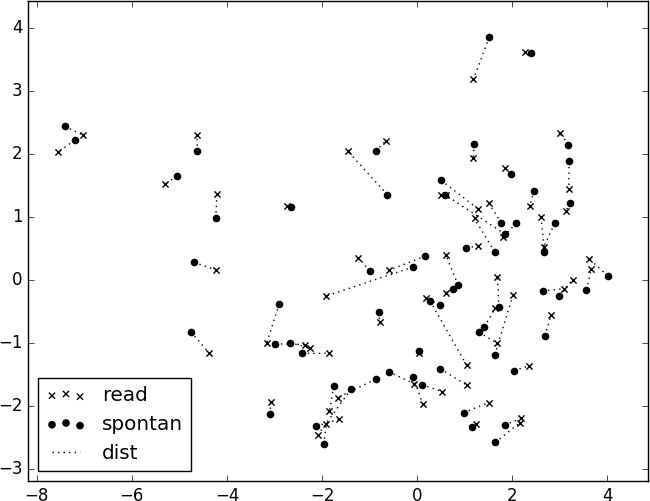
\includegraphics[width=3.25in]{perphon_dist1}
    \caption{Distances and positions of dictated-spontaneous phone pairs in 2-D space}
\label{phon_pca}
\end{figure}

\section{Utterance Classification}

General differences in spontaneous and dictated speech are observable from phoneme analysis.
Though useful for gaining insight as to why an existing model performs poorly, it would be practical to separate spontaneous and dictated speech in the absence of linguistic/grammatical information such as phones and (position in) words.
In the subsequent sections we shift the focus away from phones and the exploration of overarching differences between spontaneous and dictated speech, towards "anonymous" segments and the task of classifying spontaneous and dictated utterances.

\subsection{Segment Analysis}

Intuitively many spontaneous speech traits, such as disfluency and filled pauses, result in less constant speech rates as compared to read speech, with long segments followed by a quick succession of short segments.
In order to emulate this, a variation of the feature extraction pipeline is implemented whereby for each segment, in addition to the acoustic features, the difference in features against the preceeding segment, henceforth "delta segments", are also extracted.
In a manner similar to that of "delta-delta" MFCC features, the delta-delta segment features are also extracted.
The purpose of these features is to embed local temporal information at the segment level.
The full modified feature set is 264 features long, with both the averages and standard deviations taken for all segment features.
Table \ref{seg_feats} shows the complete list of segment acoustic features.

\begin{table}[!htb]
\renewcommand{\arraystretch}{1.3}
\caption{Modified segment-level features}
\label{seg_feats}
\centering
\begin{tabular}{l|r|r|r|r|r|r|}
    \cline{2-7}
    {} & \multicolumn{2}{|c|}{Segment}
    & \multicolumn{2}{|c|}{$\Delta$Segment}
    & \multicolumn{2}{|c|}{$\Delta\Delta$ Segment} \\
    \cline{2-7}
    {} & Mean & Std & Mean & Std & Mean & Std \\
    \hline
    \multicolumn{1}{|l|}{Duration} & 1 & 1 & 1 & 1 & 1 & 1 \\
    \hline
    \multicolumn{1}{|l|}{Log energy} & 3 & 3 & 3 & 3 & 3 & 3 \\
    \hline
    
    \multicolumn{1}{|l|}{Cepstral} & 36 & 36 & 36 & 36 & 36 & 36 \\
    \hline
    \multicolumn{1}{|l|}{Formants} & 4 & 4 & 4 & 4 & 4 & 4 \\
    \hline
\end{tabular}
\end{table}

As in the previous section, the formant and MFCC frame features are first averaged over segments.
Subsequently, the segment durations are taken, and all three components averaged over the length of the utterance.
In addition to the average, the standard deviation is also computed.
At the same time, the difference in duration, formant, and MFCC values between the currently evaluated segment and the one immediately preceeding it is calculated and the average and deviation over the utterance computed as the delta segment.
This is done once again to obtain the delta-delta segments.
In Fig. \ref{pca_delseg}, we map a sample of the utterances extracted this way into two dimensional space by Principle Component Analysis (PCA).
Although there is significant overlap in regions, the centers of each are relatively distinct, and analysis in higher dimensions may 
yield results.

\begin{figure}[!htb]
\centering
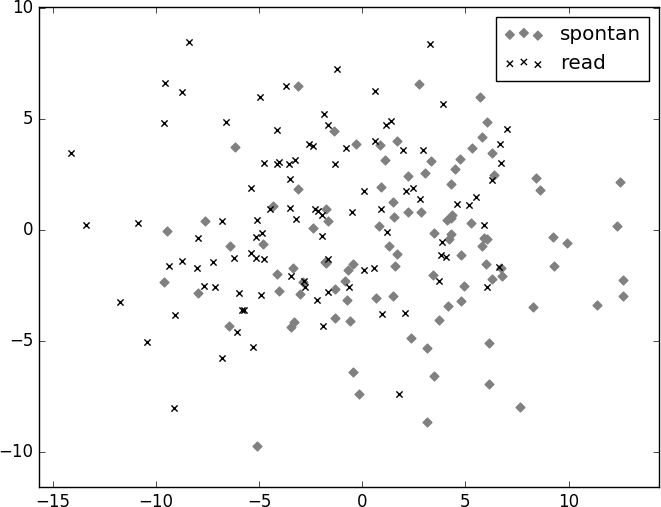
\includegraphics[width=3.25in]{pca}
    \caption{Utterance samples in 2-D space}
\label{pca_delseg}
\end{figure}

\subsection{Machine Learning and Experimentation}

An appropriate method to separate spontaneous speech is required.
As delta/delta-delta segments encode temporal information indirectly, it is difficult to utilize a sequence-sensitive method such as a Markov Process.
Hence, general approaches such as ensemble methods, Support Vector Machines (SVM), and logistic regression are considered instead.

Ensemble methods employ a large number of weak classifiers built on a particular learning algorithm and combine their predictions in order to improve generalizability and robustness.
A random forest is similar to a classification tree, differing in the branching behavior.
While in decision/classification tree learning the best predictor (the one that most separates the data) is taken, in random forests a random sample of the predictors is taken instead, and the best split chosen from it \cite{liaw}.

A training pipeline is built utilizing the Python scientific stack, with feature extraction and data analysis methods built on Pandas and cross validation, classification, and evaluation provided by Scikit-Learn \cite{sklearn}.
Instead of processing data iteratively, the dataset is processed in parallel utilizing the distributed capabilities of Dask and Pandas.

\section{Results and Analysis}

An equal number of positive (spontaneous) and negative (read) utterances are sampled and trained on a number of classifiers.
The initial classification results, evaluated by average accuracy, F1 scores, and their respective standard deviations over ten folds, are shown in Table \ref{init_results}.
The classifiers considered here are Stochastic Gradient Descent (SGD) classfiers utilizing the Support Vector Machine (SVM) and logistic regression (Log) loss functions, resepectively, and ensemble methods consisting of random forest (R.Forest) and gradient boosting (G.Boost) classification.
Ten-fold cross validation on shuffled data is used throughout, with the full feature set utilized to obtain the initial results.

\begin{table}[!htb]
\renewcommand{\arraystretch}{1.3}
    \caption{Initial classification results}
\label{init_results}
\centering
\begin{tabular}{l|rr|rr}
    {} & \multicolumn{2}{|c|}{Accuracy} &
    \multicolumn{2}{|c}{F1 score} \\
    {} & Mean & Std & Mean & Std \\
    \hline
    SVM &  0.906142 &  0.012277 &  0.906234 &  0.015051 \\
    Log &  0.907956 &  0.007953 &  0.907332 &  0.010498 \\
    R.Forest &  0.928603 &  0.008885 &  0.931077 &  0.007835 \\
    G.Boost &  0.939792 &  0.010555 &  0.938142 &  0.008998 \\
\end{tabular}
\end{table}

The nearly identical accuracy and F1 scores for each method indicates that classification accuracy between spontaneous and dictated speech is nearly equal.
However, upon closer inspection classification results are consistently worse for spontaneous speech.
This is to be expected given the higher variability of spontaneous speech and given that training was conducted on equal amounts of spontaneous and dictated data.
On the other hand, this should be somewhat offset by the larger average number of segments per utterance for spontaneous speech in the corpus.

Fig. \ref{hit_rate} displays the "hit rate" of the random forest classifier trained previously.
This is the squared ratio between the number of hits (correct predictions) and misses (incorrect predictions) given the number of segments in an utterance.
Similar results were achieved with the other classifiers.
In general, longer utterances produce higher hit rates, indicating classification success.
It must be noted that utterance length itself should not be and is not used as a feature, as the length of read utterances are predicated during the design of the prepared text and hence not necessarily indicative of any real world differences between spontaneous and read speech.
Still, given the large difference in the number of segments per utterance between read and spontaneous speech in this particular corpus, there is the danger that results will not generalize in real-world cases.
Further studies with different datasets must be conducted to investigate the applicability of these findings.

\begin{figure}[!htb]
\centering
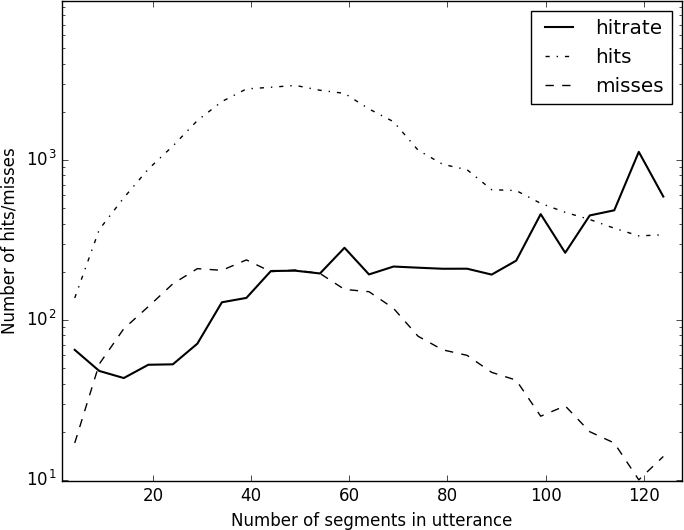
\includegraphics[width=3.2in]{hitrate}
    \caption{Number of hits and misses against utterance length}
\label{hit_rate}
\end{figure}

The random forest classifier, possessing the lowest standard deviation of all tested methods, is further tweaked.
Parameter tuning is done by first extracting the relative importance of the features utilized previously.
The relative importance of a feature measures the fraction of all training examples classified by it.
Of the initial training examples, 44.7\% of the utterances were classified by the six durational and eighteen log energy features, contributing 24.370\%, 9.725\%, 7.0291\%, and 4.8284\% respectively.
Training on the reduced feature set leads to a very slight improvement in accuracy (93.27\%) and F1 scores (93.23\%) and a large reduction in training times.
On the reduced feature set, the most relatively important features are the average delta and delta-delta segment duration features at 17.2\% and 14.8\% respectively, followed by the average delta segment log energy at 7.7\% and deviation delta segment duration at 7.0\%.
Iteratively combining the remaining features and re-training the classifier lead to no further accuracy gains.

\section{Conclusion and future works}

There are distinguishable differences in the acoustic characteristics of Indonesian phonemes between spontaneous and read speech.
Measured by phoneme duration, log energy levels, and occurence distribution, there are observable differences in many common vowels and also plosives and fricatives.
Exploring methods to better represent these phonemes in training data, both in terms of occurence frequency and acoustic characterisitics, may improve speech recognition performance.
In the future, a method to suggest improvements to the existing corpus building process based on these findings would be beneficial.

Preliminary results suggest that delta and delta-delta segment information are promising features in the classification of utterances into spontaneous and dictated Indonesian speech.
On a cross-validated training set, F1 scores of 93.23\% were achieved on a random forest classifier utilizing a feature set consisting of 24 values; the averages and deviations of segment duration and energy, delta segment duration and energy, and delta-delta segment duration and engery.
Classification results above 90\% were achieved across all tested classifiers.
Further research is needed to determine if this holds true for other datasets and in different acoustic conditions.
If robust, this approach may be useful for multi-class classification tasks such as dialect and speaking style classification, or as a front-end to switch between various specialized back-end models.

\section*{Acknowledgements}

This research is partially supported by “Riset Unggulan
Perguruan Tinggi Kemenristekdikti” (University
Distinguished Research) and is part of a larger project titled
“Pengembangan Perangkat Lunak Perisalah Rapat dengan
Memanfaatkan Teknologi Pengenal Ucapan, Mesin Translasi,
dan Peringkas Otomatis” (Development of Meeting Speech
Transcriber Using Speech Recognition, Machine Translation,
and Automatic Summarizer Technology). We also would like
to thank PT INTI, Bandung, Indonesia for the utilization of
the speech corpus presented in this research.

\begin{thebibliography}{1}

\bibitem{hoesen}
D.~Hoesen, C.~Satriawan, D.P.~Lestari, M.L.~Khodra,
    "Toward Robust Indonesian Speech Recognition with Spontaneous-speech Adapted Acoustic Models,"
    SLTU-2016 5th Workshop on Spoken Language Technologies for under-resourced languages, 2016.

\bibitem{lestari}
D.P.~Lestari, K.~Iwano, S.~Furui,
    "A large vocabulary continuous speech recognition system for Indonesian language,"
    Proc. 15th Indonesian Scientific Conference in Japan, 2006.

\bibitem{barik}
H.C.~Barik, 
    "Cross-linguistic study of temporal characteristics of different types of speech material,"
    Language and Speech 20, pp. 116-126, 1977.

\bibitem{blaauw}
E.~Blaauw,
    "The contribution of prosodic boundary markers to the perceptual difference between read and spontaneous speech,"
    Speech Communications 14(4), pp. 359-375, 1995.

\bibitem{umeda}
N.~Umeda, K.~Wallace, K.~Horna,
    "Usage of words and sentence structures in spontaneous versus text material,"
    Proc. ICSLP vol.1, pp. 759-762, 1992.

\bibitem{lestari2}
D.P.~Lestari, A.~Irfani,
    "Acoustic and Language Model Adaptation for Indonesian Spontaneous Speech Recognition,"
    2nd International Conference on Advanced Informatics: Concepts, Theory, and Application (ICAICTA), 2015.

\bibitem{sakti}
S.~Sakti et al,
    "Development of Indonesian large vocabulary continuous speech recognition system with A-STAR project,"
    Proc. of the Workshop on TCAST, pp. 19, 2008.

\bibitem{sani}
A.~Sani, D.P.~Lestari, A.~Purwarianti,
    "Filled Pause Detection in Indonesian Spontaneous Speech,"
    Communications in Computer and Information Science vol. 293, pp. 54-64, 2016.

\bibitem{laan}
G.P.M.~Laan,
    "The contributions of intonation, segmental durations, and spectral features to the perception of a spontaneous and a read speaking style,"
    Speech Communication 22:43-65, 1997.

\bibitem{dellwo}
V.~Delwo, A.~Leemann, M.J.~Kolly,
    "The recognition of read and spontaneous speech in local vernacular: The case of Zurich German,"
    Journal of Phonetics vol. 48, 2015, pp. 13-28.

\bibitem{silverman}
K.~Silverman, E.~Blaauw, J.~Spitz, J.~Pitrelli,
    "Towards Using Prosody in Speech Recognition/Understanding Systems: Differences Between Read and Spontaneous Speech",

\bibitem{liu}
G.~Liu, Y.~Lei, J.H.L.~Hansen,
    "Dialect Identification: Impact of Differences Between Read and Spontaneous Speech",
    18th European Signal Processing Conference (EUISPCO-2010), 2010.

\bibitem{furui1}
S.~Furui, M.~Nakamura, T.~Ichiba, K.~Iwano,
	"Why is the recognition of spontaneous speech so hard?",
	8th Internation Conference on Text, Speech, and Dialog,
	Karlovy Vary, 2005.

\bibitem{povey}
D.~Povey, et al.,
    "The Kaldi speech recognition toolkit,"
    IEEE Workshop on ASRU, 2011.

\bibitem{furui2}
S.~Furui,
    "Recent advances in spontaneous speech recognition and understanding",
    Proc. IEEE Workshop on Spontaneous Speech Processing and Recognition, pp. 1-6, 2003.

\bibitem{benzeguiba}
M.~Benzeguiba, R.~DeMori, O.~Deroo, S.~Dupon, T.~Erbes, D.~Jouvet, L.~Fissore, P.~Laface, A.~Mertins, C.~Ris, R.~Rose, V.~Tyagi, C.~Wellekens,
	"Automatic Speech Recognition and Speech Variability: a Review",
	Speech Communication 49:763-786, 2007.

\bibitem{asami}
T.~Asami, R.~Masamura, H.~Masataki, S.~Sakauchi,
    "Read and spontaneous speech classification based on variance of GMM supervectors",
	Interspeech 2014:2375-2379, 2014.

\bibitem{nakamura}
M.~Nakamura, I.~Koji, S.~Furui,
    "Differences between acoustic characteristics of spontaneous and read speech and their effects on speech recognition performance",
    Computer Speech and Language 22(2): 171-184, 2008.

\bibitem{scharenborg}
O.~Scharenborg, V.~Wan, M.~Ernestus
    "Unsupervised speech segmentation: An analysis of the hypothesized phone boundaries,"
    Journal of the Acoustical Society of America 127:1084-1095, 2010.

\bibitem{sklearn}
F.~Pedregosa et al.,
    "Scikit-learn: Machine learning in Python,"
    The Journal of Machine Learning Research 12 (2011): 2825-2830.

\bibitem{liaw}
A.~Liaw, M.~Weiner,
    "Classification and Regression by randomForest,"
    R News 2(3), 18-22, 2002.

\end{thebibliography}



% CONTEKAN:


% An example of a floating figure using the graphicx package.
% Note that \label must occur AFTER (or within) \caption.
% For figures, \caption should occur after the \includegraphics.
% Note that IEEEtran v1.7 and later has special internal code that
% is designed to preserve the operation of \label within \caption
% even when the captionsoff option is in effect. However, because
% of issues like this, it may be the safest practice to put all your
% \label just after \caption rather than within \caption{}.
%
% Reminder: the "draftcls" or "draftclsnofoot", not "draft", class
% option should be used if it is desired that the figures are to be
% displayed while in draft mode.
%
%\begin{figure}[!t]
%\centering
%\includegraphics[width=2.5in]{myfigure}
% where an .eps filename suffix will be assumed under latex, 
% and a .pdf suffix will be assumed for pdflatex; or what has been declared
% via \DeclareGraphicsExtensions.
%\caption{Simulation results for the network.}
%\label{fig_sim}
%\end{figure}

% Note that the IEEE typically puts floats only at the top, even when this
% results in a large percentage of a column being occupied by floats.


% An example of a double column floating figure using two subfigures.
% (The subfig.sty package must be loaded for this to work.)
% The subfigure \label commands are set within each subfloat command,
% and the \label for the overall figure must come after \caption.
% \hfil is used as a separator to get equal spacing.
% Watch out that the combined width of all the subfigures on a 
% line do not exceed the text width or a line break will occur.
%
%\begin{figure*}[!t]
%\centering
%\subfloat[Case I]{\includegraphics[width=2.5in]{box}%
%\label{fig_first_case}}
%\hfil
%\subfloat[Case II]{\includegraphics[width=2.5in]{box}%
%\label{fig_second_case}}
%\caption{Simulation results for the network.}
%\label{fig_sim}
%\end{figure*}
%
% Note that often IEEE papers with subfigures do not employ subfigure
% captions (using the optional argument to \subfloat[]), but instead will
% reference/describe all of them (a), (b), etc., within the main caption.
% Be aware that for subfig.sty to generate the (a), (b), etc., subfigure
% labels, the optional argument to \subfloat must be present. If a
% subcaption is not desired, just leave its contents blank,
% e.g., \subfloat[].


% An example of a floating table. Note that, for IEEE style tables, the
% \caption command should come BEFORE the table and, given that table
% captions serve much like titles, are usually capitalized except for words
% such as a, an, and, as, at, but, by, for, in, nor, of, on, or, the, to
% and up, which are usually not capitalized unless they are the first or
% last word of the caption. Table text will default to \footnotesize as
% the IEEE normally uses this smaller font for tables.
% The \label must come after \caption as always.
%
%\begin{table}[!t]
%% increase table row spacing, adjust to taste
%\renewcommand{\arraystretch}{1.3}
% if using array.sty, it might be a good idea to tweak the value of
% \extrarowheight as needed to properly center the text within the cells
%\caption{An Example of a Table}
%\label{table_example}
%\centering
%% Some packages, such as MDW tools, offer better commands for making tables
%% than the plain LaTeX2e tabular which is used here.
%\begin{tabular}{|c||c|}
%\hline
%One & Two\\
%\hline
%Three & Four\\
%\hline
%\end{tabular}
%\end{table}


% Note that the IEEE does not put floats in the very first column
% - or typically anywhere on the first page for that matter. Also,
% in-text middle ("here") positioning is typically not used, but it
% is allowed and encouraged for Computer Society conferences (but
% not Computer Society journals). Most IEEE journals/conferences use
% top floats exclusively. 
% Note that, LaTeX2e, unlike IEEE journals/conferences, places
% footnotes above bottom floats. This can be corrected via the
% \fnbelowfloat command of the stfloats package.



% trigger a \newpage just before the given reference
% number - used to balance the columns on the last page
% adjust value as needed - may need to be readjusted if
% the document is modified later
%\IEEEtriggeratref{8}
% The "triggered" command can be changed if desired:
%\IEEEtriggercmd{\enlargethispage{-5in}}



% that's all folks
\end{document}


